\documentclass[12pt]{article}
\usepackage[english]{babel}
\usepackage[square,numbers]{natbib}
\bibliographystyle{abbrvnat}
\usepackage{url}
\usepackage[utf8x]{inputenc}
\usepackage{amsmath}
\usepackage{graphicx}
\usepackage{booktabs}
\graphicspath{{images/}}
\usepackage{parskip}
\usepackage{fancyhdr}
\usepackage{vmargin}
\usepackage[section]{placeins}

\usepackage{tabularx}

\setmarginsrb{3 cm}{2.5 cm}{3 cm}{2.5 cm}{1 cm}{1.5 cm}{1 cm}{1.5 cm}

\title{Investigating Properties of Houses from a New York Airbnb Dataset}                             % Title
\author{Edward Yidong FANG}                               % Author
\date{\today}                                           % Date

\makeatletter
\let\thetitle\@title
\let\theauthor\@author
\let\thedate\@date
\makeatother

\pagestyle{fancy}
\fancyhf{}
\rhead{\theauthor}
\lhead{Intelligent Data Analysis}
\cfoot{\thepage}

\begin{document}

%%%%%%%%%%%%%%%%%%%%%%%%%%%%%%%%%%%%%%%%%%%%%%%%%%%%%%%%%%%%%%%%%%%%%%%%%%%%%%%%%%%%%%%%%

\begin{titlepage}
    \centering
    \vspace*{0.5 cm}
    
\includegraphics[width=0.3\textwidth, trim = {0 90px 0 0}, clip]{images/sustclogo.png}\\[0.0 cm]   % University Logo
    \textsc{\Large Southern University of Science and Technology}\\[2.0 cm]  
    \textsc{\Large CS212 Intelligent Data Analysis}\\[0.5 cm]               
    \large Director: Prof. Peter Ti\v{n}o\\[0.5 cm]             
    \rule{\linewidth}{0.2 mm} \\[0.4 cm]
    { \huge \bfseries \thetitle}\\
    \rule{\linewidth}{0.2 mm} \\[1.5 cm]
    
    \begin{minipage}{0.4\textwidth}
        \begin{flushleft} \large
            \emph{Author:}\\
            \theauthor
            \end{flushleft}
            \end{minipage}~
            \begin{minipage}{0.4\textwidth}
            \begin{flushright} \large
            \emph{Student Number:} \\
            11510493                                   % Your Student Number
        \end{flushright}
    \end{minipage}\\[1 cm]
    Email: 11510493@mail.sustc.edu.cn\\[1 cm]
    {\large Shenzhen, China \thedate}\\[2 cm]
    \vfill
\end{titlepage}
\begin{abstract}
   In these experiments, three basic methods of data analysis are implemented, which is Principle Components Anaylysis (PCA), Clustering and Self-organizing Map (SOM). By applying there methods, the relations among different attributes are discussed. After the dimension reduction, it was found that the attributes can be predicted by others to some extent, while some can not. The relations will be presented mostly as different firgures.
\end{abstract}
%%%%%%%%%%%%%%%%%%%%%%%%%%%%%%%%%%%%%%%%%%%%%%%%%%%%%%%%%%%%%%%%%%%%%%%%%%%%%%%%%%%%%%%%
\tableofcontents
\pagebreak
%%%%%%%%%%%%%%%%%%%%%%%%%%%%%%%%%%%%%%%%%%%%%%%%%%%%%%%%%%%%%%%%%%%%%%%%%%%%%%%%%%%%%%%%
\section{Introduction}
Airbnb is an online marketplace and hospitality service, enabling people to lease or rent short-term lodging including vacation rentals, apartment rentals, homestays, hostel beds, or hotel rooms. The dataset analysed in there experiments is derived from Tom Slee's blog\cite{slee-2017} and it is crawled from the website of Airbnb. And only a small part of data for New York, crawled on 05/06/2017, are analysed.

\section{Data Preprocessing}
\subsection{Data Description}
Here is the meaning for each column in the collected CSV file:
\begin{itemize}
\item room\_id: A unique number identifying an Airbnb listing. The listing has a URL on the Airbnb web site of \url{http://airbnb.com/rooms/room_id}
\item survey\_id: A unique number identifying the behaviour of survey.
\item host\_id: A unique number identifying an Airbnb host. The host’s page has a URL on the Airbnb web site of \url{http://airbnb.com/users/show/host_id}
\item room\_type: One of “Entire home/apt”, “Private room”, or “Shared room”
\item country: the nation the room located in; acutually no data
\item city: the city the room located in
\item borough: A subregion of the city or search area for which the survey is carried out. The borough is taken from a shapefile of the
city that is obtained independently of the Airbnb web site. For some cities, there is no borough information; for others the borough may be a number. If you have better shapefiles for a city of interest, please send them to me.
\item neighborhood: As with borough: a subregion of the city or search area for which the survey is carried out. For cities that have both, a neighbourhood is smaller than a borough. For some cities there is no neighbourhood information.
\item reviews: The number of reviews that a listing has received. Airbnb has said that 70\% of visits end up with a review, so the number of reviews can be used to estimate the number of visits. Note that such an estimate will not be reliable for an individual listing (especially as reviews occasionally vanish from the site), but over a city as a whole it should be a useful metric of traffic.
\item overall\_satisfaction: The average rating (out of five) that the listing has received from those visitors who left a review.
\item accommodates: The number of guests a listing can accommodate.
\item bedrooms: The number of bedrooms a listing offers.
\item bathrooms: The number of bathrooms a listing offers, actually not available.
\item price: The price (in \$US) for a night stay.
\item minstay: The minimum stay for a visit, as posted by the host.
\item name: The name of the room.
\item property\_type:“Apartment”, “Loft”, “Villa”, “House”, etc.
\item latitude and longitude: The latitude and longitude of the listing as posted on the Airbnb site: this may be off by a few hundred metres. 
\item last\_modified: the date and time that the values were read from the Airbnb web site.
\item location: Unkown, certain number related to the location of the room.
\end{itemize}
The first line of the CSV file holds the column headings.
\subsection{Data Preprocessing}
Note that in this report only the data preprocessing process of the first problem is shown, but the other data preprocessing processes are all very similar.
\subsubsection{Removing of the useless data and the Selection of the records}

As the amount of data is really large (up to 40,730 rows), we just remove the data records without avaiable \textit{reviews} or \textit{overrall\_satisfaction}. Since the prices higher than \$200 per night are assumed as not reasonable, the records with those extremely high prices are removed. 
 Also, as the columns \textit{room\_id, survey\_id, host\_id, country, city, last\_modified} and \textit{location} are meaningless, we removed them from the data. In addition, it is found that the values of column \textit{bathrooms} and \textit{minstay} are unavailable.
\par
Finally, for the simplification of the problem, we just retrieve the records whose boroughs are “Manhattan” or ``Brooklyn''. And the experimental data are sampled from the original data under the sample fraction of $0.1$.\par

\begin{table}[h]
\resizebox{\linewidth}{!}{
\begin{tabular}{lllrrrrrrrl}
\toprule
{} &        room\_type &    borough &  accommodates &  reviews &  overall\_satisfaction &  bedrooms &  price &  longitude &   latitude & property\_type \\
\midrule
0 &  Entire home/apt &   Brooklyn &             2 &       95 &                   5.0 &       0.0 &  125.0 & -73.943276 &  40.721256 &     Apartment \\
1 &  Entire home/apt &   Brooklyn &             3 &        3 &                   4.5 &       1.0 &  165.0 & -73.952168 &  40.723975 &         House \\
2 &  Entire home/apt &  Manhattan &             5 &       25 &                   4.0 &       2.0 &  220.0 & -73.962862 &  40.758275 &     Apartment \\
3 &  Entire home/apt &  Manhattan &             2 &        2 &                   0.0 &       1.0 &  180.0 & -74.003905 &  40.733196 &     Apartment \\
4 &  Entire home/apt &   Brooklyn &             4 &        3 &                   5.0 &       1.0 &  132.0 & -73.957279 &  40.733538 &     Apartment \\
\bottomrule
\end{tabular}
}
    \caption{Data After preprocessing}
    \label{tab:data1}
\end{table}
The data at the end looks like the Table \ref{tab:data1}.\\
\subsubsection{One Hot Encoding}
To make use of the data field \textit{room\_type}, \textit{borough} and \textit{property\_type}, both of the infomation are encoded using the method called One-Hot encoding to transform the data. By doing so, it is ensured that the infomation of all possible aspects of the room are included into the data matrix.\\
For example, if there two roon, whose types are ``Private room'' and ``Entire home/apt'', respectively, then the encoded result looks like Table \ref{tab:onehot}. Three different columns are added to enumerate all possible room types. And the values are all zeros except for the room type the room belongs to.
\begin{table}[h]
\resizebox{\linewidth}{!}{
\begin{tabular}{lrrrrrrrrr}
\toprule
{} &  accommodates &  ...  &   latitude &  room\_type\_Entire home/apt &  room\_type\_Private room &  room\_type\_Shared room &...\\
\midrule
0 &             2 &...&   40.691398 &                          0 &                       1 &                      0 &...\\
1 &             4 &...&  40.811016 &                          1 &                       0 &                      0 &...\\
\bottomrule
\end{tabular}}
\caption{Example Data After One-hot Encoding}
    \label{tab:onehot}
\end{table}
\subsubsection{Data Standardization}
To see the significance of data standardization, two box plot was made, one for the raw data and another for the standardized data. Note that the one-hot encoded columns are standardized but are not included in the figures because the scal of the box plot will be influenced by those attributes and make the differece hard to distinguish.\\
\begin{figure}[htbp]
\centering
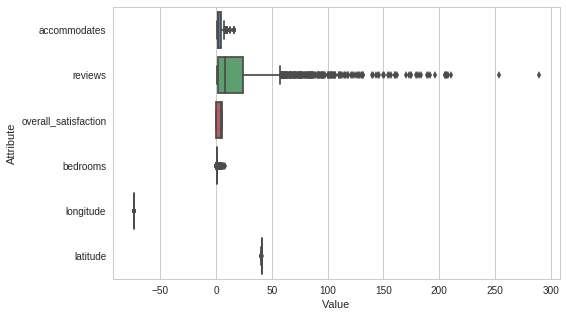
\includegraphics[width = \textwidth]{images/before-std.png}
\caption{Data before standardization}
\label{fig:before-std}
\end{figure}
As is obvious from the Figure \ref{fig:before-std}, the values of attribute \textit{reviews} are not in the same scale with other attributes. Neither does the longtitude and latitude. If we use these values in the matrix we will calculate later, the importance of attribute \textit{reviews} ,\textit{latitude} and \textit{longtitude} will be extremly larger than ohter attributes. Thus, we need to apply the standardization to the raw data.

\par Standardization can be done in many ways, the formula
\[NewValue = (OldValue-Mean)/StandardDeviation\]
is enough for this dataset. The result is shown in the Figure \ref{fig:after-std}.
\begin{figure}[htbp]
\centering
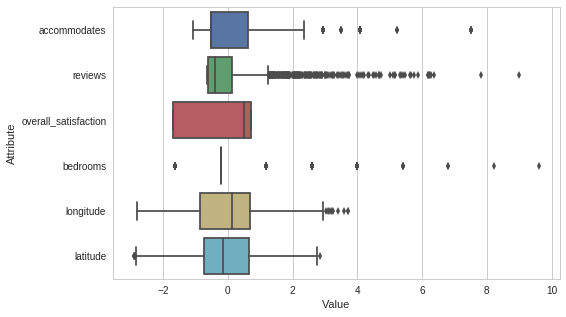
\includegraphics[width = \textwidth]{images/after-std.png}
\caption{Data after standardization}
\label{fig:after-std}
\end{figure}
\section{Questions to Ask and Labeling}
\subsection{Questions to Ask}

When people go out and want to find a room to stay in a city, it can be said that the most concerning aspects of a room is its condition, position and price. In the dataset analysed, the price is already there and the overall satisfaction can represent a combination of all the aspects. Thus, two questions are going to be explored in these expriment.
\begin{itemize}
\item Can the ranges of price be roughly predicted using other attributes of the data?
\item Can the overall stasfications be roughly predicted using other attributes of data?
\item What is the most crucial factors that influence the price and overall satisfaction among the attributes we have?

\item How much the difference will be for the data in two different borough?
\end{itemize}
\subsection{Labeling Schemes}
\subsubsection{Label of Prices}
\begin{figure}[htb]
\centering
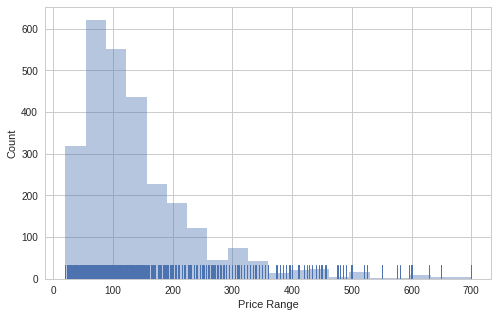
\includegraphics[width = 0.8\textwidth]{images/price-distr.png}
\caption{Distribution of prices that is lower than \$750}
\label{fig:price-distr}
\end{figure}
The price level can be classify into three level according to the distribution of the prices. Fig.\ref{fig:price-distr} shows the distribution and according to it, the data are labelled into three approximately-equal-size classes: ``low price'', ``middle price'' and ``high price''.\par
 Note that for the convenience of visualization, we just plot the distribution of prices that is lower than \$750, and only a few records' prices are higher than \$750.
 \par
 After some trying, it is finnally found that these three intervals are best for the data to be evenly devided and labelled: \([0,85)\), \([85, 149)\) and \([149, \infty)\).
\subsubsection{Label of Overall Satisfaction}
The label of overall satisfication is set to be ``low'' if \textit{overall\_satisfaction} is equal to or less than 4, ``median'' if is equal to 4.5, ``high'' if equal to 5.
\section{Data Analysis}
After the preprocessing of the data, the Principle Component Anaylysis (PCA) algorithm was used to generate the eigenvalues, eigenvectors, and coefficients to the eigenvalues, which actually are the variances that contianed in each directions that eigenvectors expend.
\subsection{Coordinate Projections}
%%%%%%%%%%%%%%%%%%%%%%%%%%%%%%%%% figures %%%%%%%%%%%%%%%%%%%%%%%%%%%%%%%%%%%%%%%
First some simple projections of just two attribues of the data are used.\\
As most of our attributes are discrete, some of the important can be distinguished as a form of points' labels.  
\\ From most of these figures such as Fig.\ref{fig:pair-acc-price} and Fig.\ref{fig:pair-bedrooms-price} it can be found that the average room price in Manhattan is generally higher than that in Brookly. This is perhaps due to the fact that Manhattan is the center of the city. Also, Fig.\ref{fig:pair-acc-price} indicates that the larger the accomodates number is, the higher the price is. The trend of price over number of bedrooms in Fig.\ref{fig:pair-bedrooms-price} is similar, which is intutively true.
\par However, Fig. \ref{fig:pair-latitude-longitude-price}, \ref{fig:pair-over-price1}, \ref{fig:pair-over-price2}, \ref{fig:pair-reviews-price1} and \ref{fig:pair-reviews-price2} also show some relation  between price and location, overall satisfication, room type and reviews number. So which of there attributes can influence the price mostly, i.e. the importance of these attributes. Then it can be figured out by the technique of PCA.
\begin{figure}[htb]
\centering
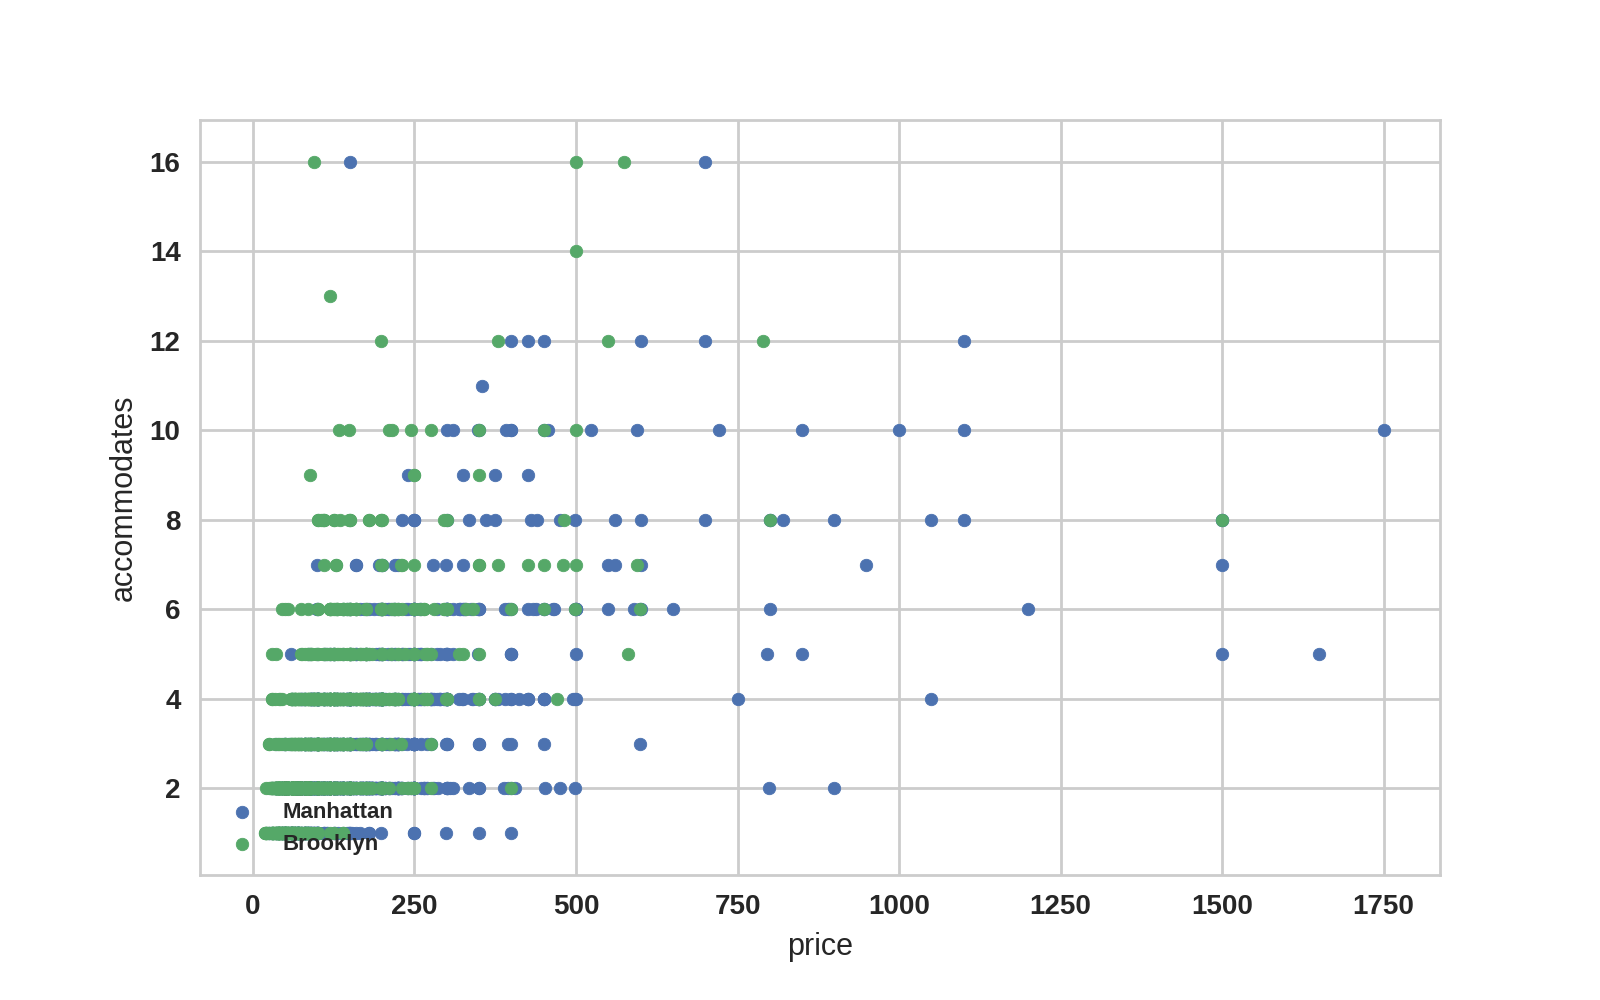
\includegraphics[width = 0.8\textwidth]{images/pair-acc-price.png}
\caption{A 2D-projection on to the prices and accomdates with borough label}
\label{fig:pair-acc-price}label{fig:pair-over-price2}
\end{figure}
\begin{figure}[htb]
\centering
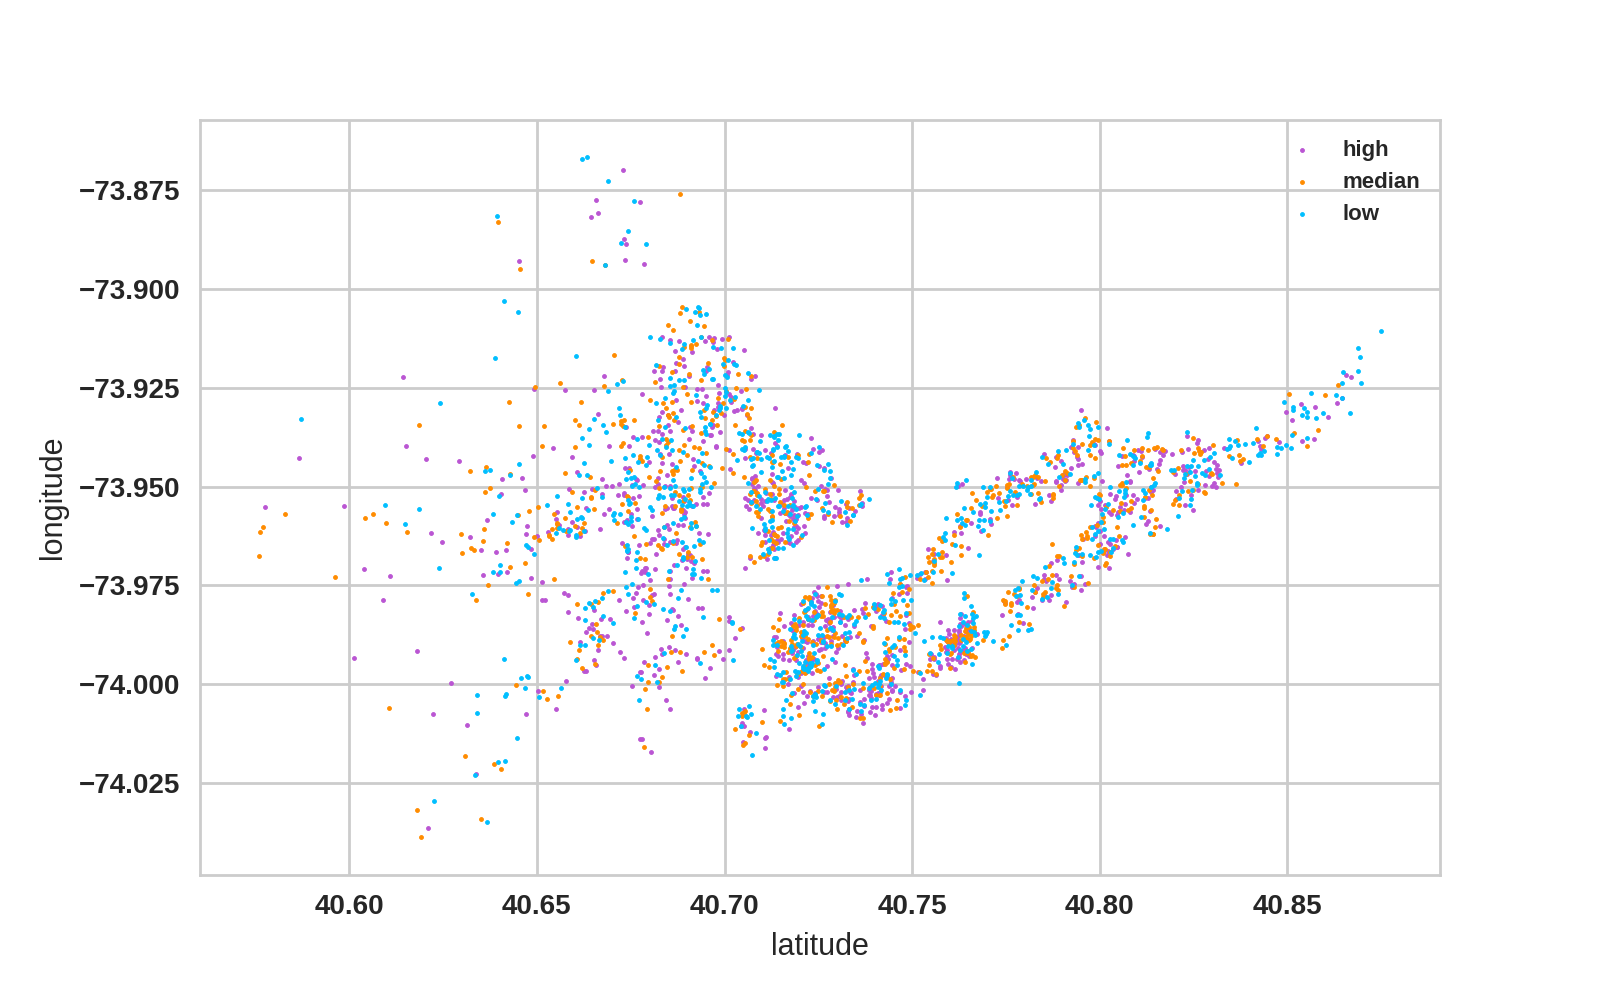
\includegraphics[width = 0.8\textwidth]{images/pair-bedrooms-price.png}
\caption{A 2D-projection on to the prices and bedrooms with borough label}
\label{fig:pair-bedrooms-price}
\end{figure}
\begin{figure}[htb]
\centering
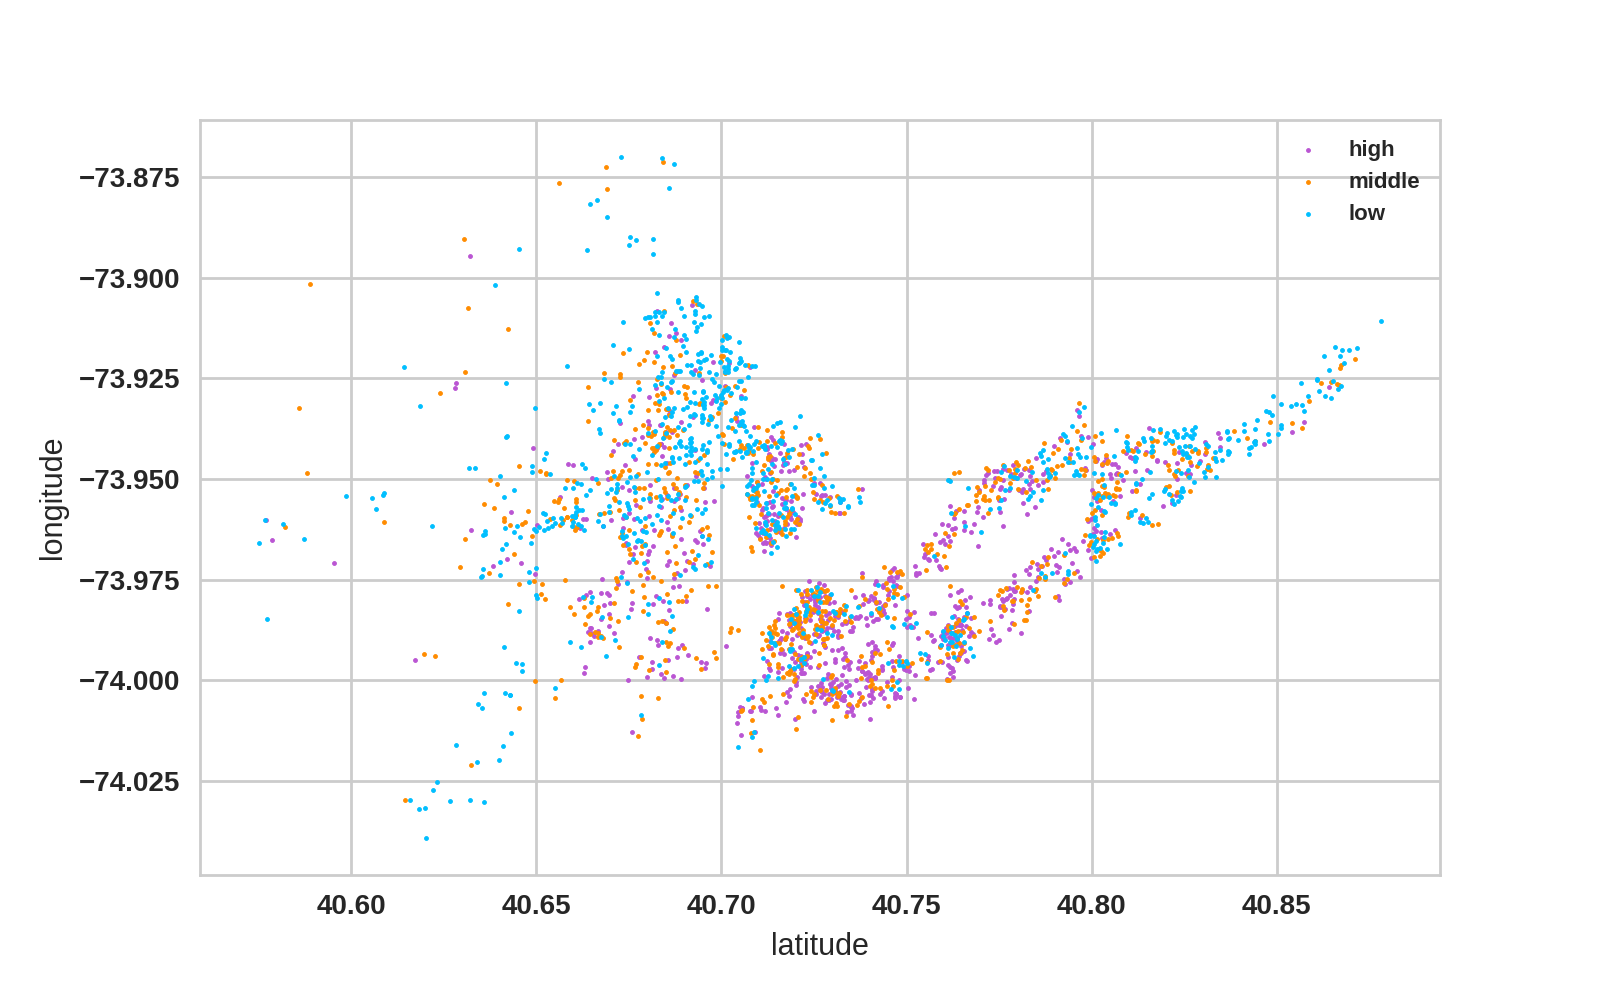
\includegraphics[width = 0.8\textwidth]{images/pair-latitude-longitude-price.png}
\caption{A 2D-projection on to the latitude and longitude with price label}
\label{fig:pair-latitude-longitude-price}
\end{figure}

\begin{figure}[htb]
\centering
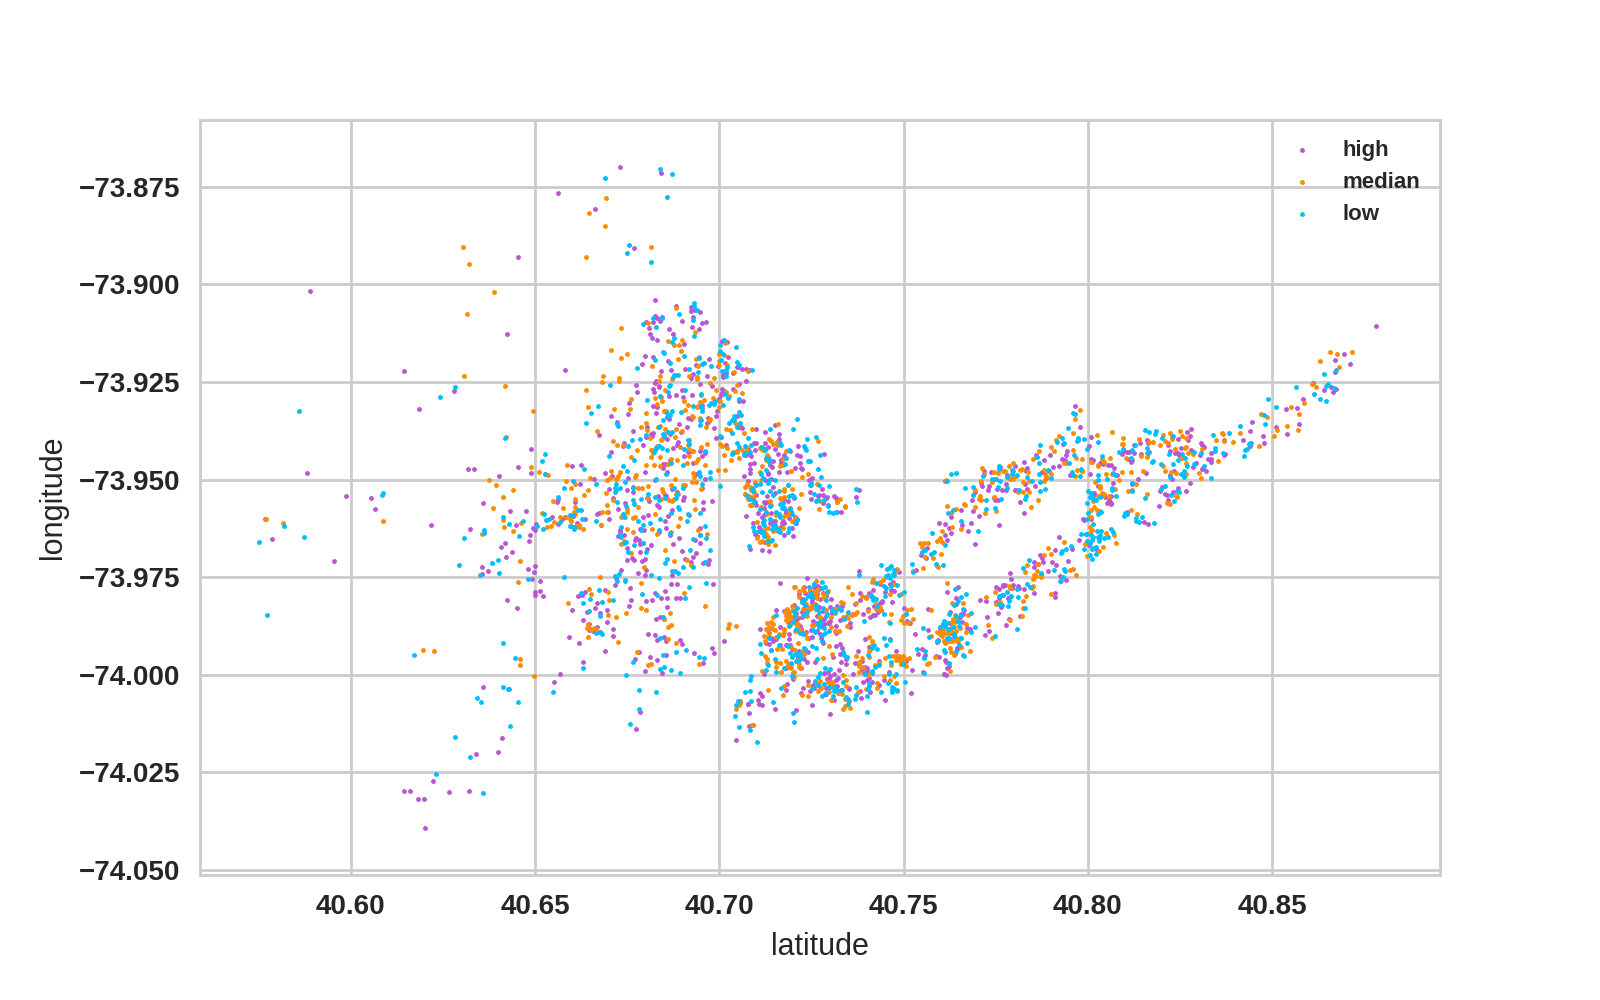
\includegraphics[width = 0.8\textwidth]{images/pair-latitude-longitude-satisfiction.png}
\caption{A 2D-projection on to the latitude and longitude with satisfiction label}
\label{fig:pair-latitude-longitude-satisfiction}
\end{figure}
\begin{figure}[htb]
\centering
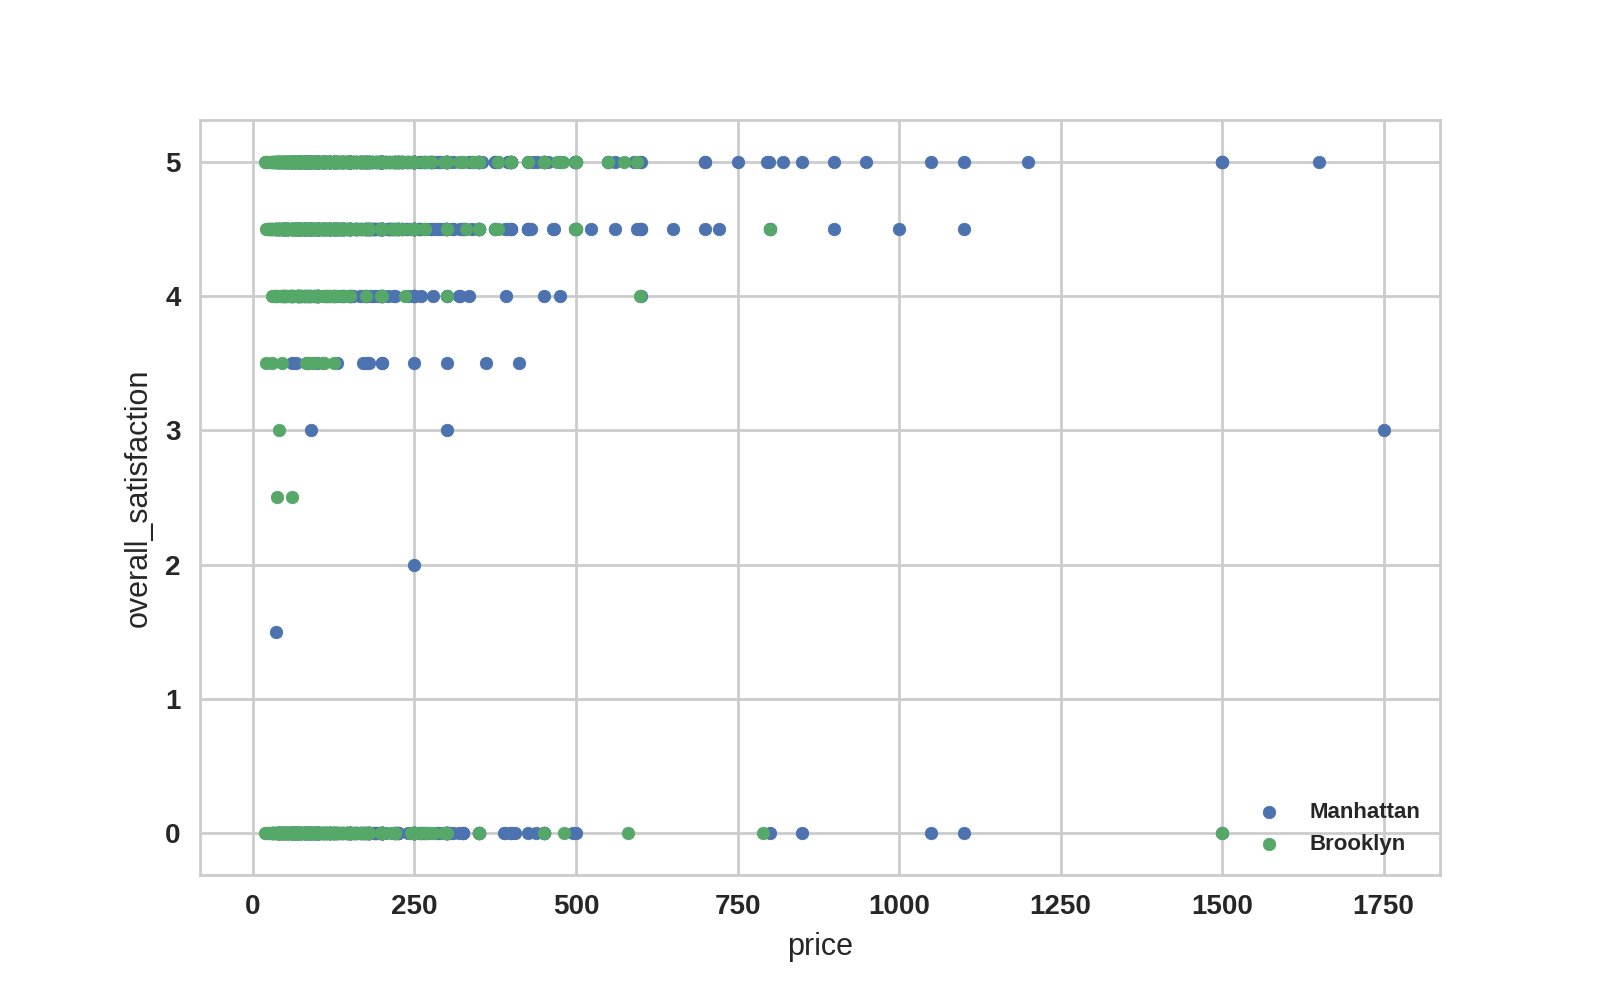
\includegraphics[width = 0.8\textwidth]{images/pair-over-price1.png}
\caption{A 2D-projection on to the satisfiction and price with borough label}
\label{fig:pair-over-price1}
\end{figure}
\begin{figure}[htb]
\centering
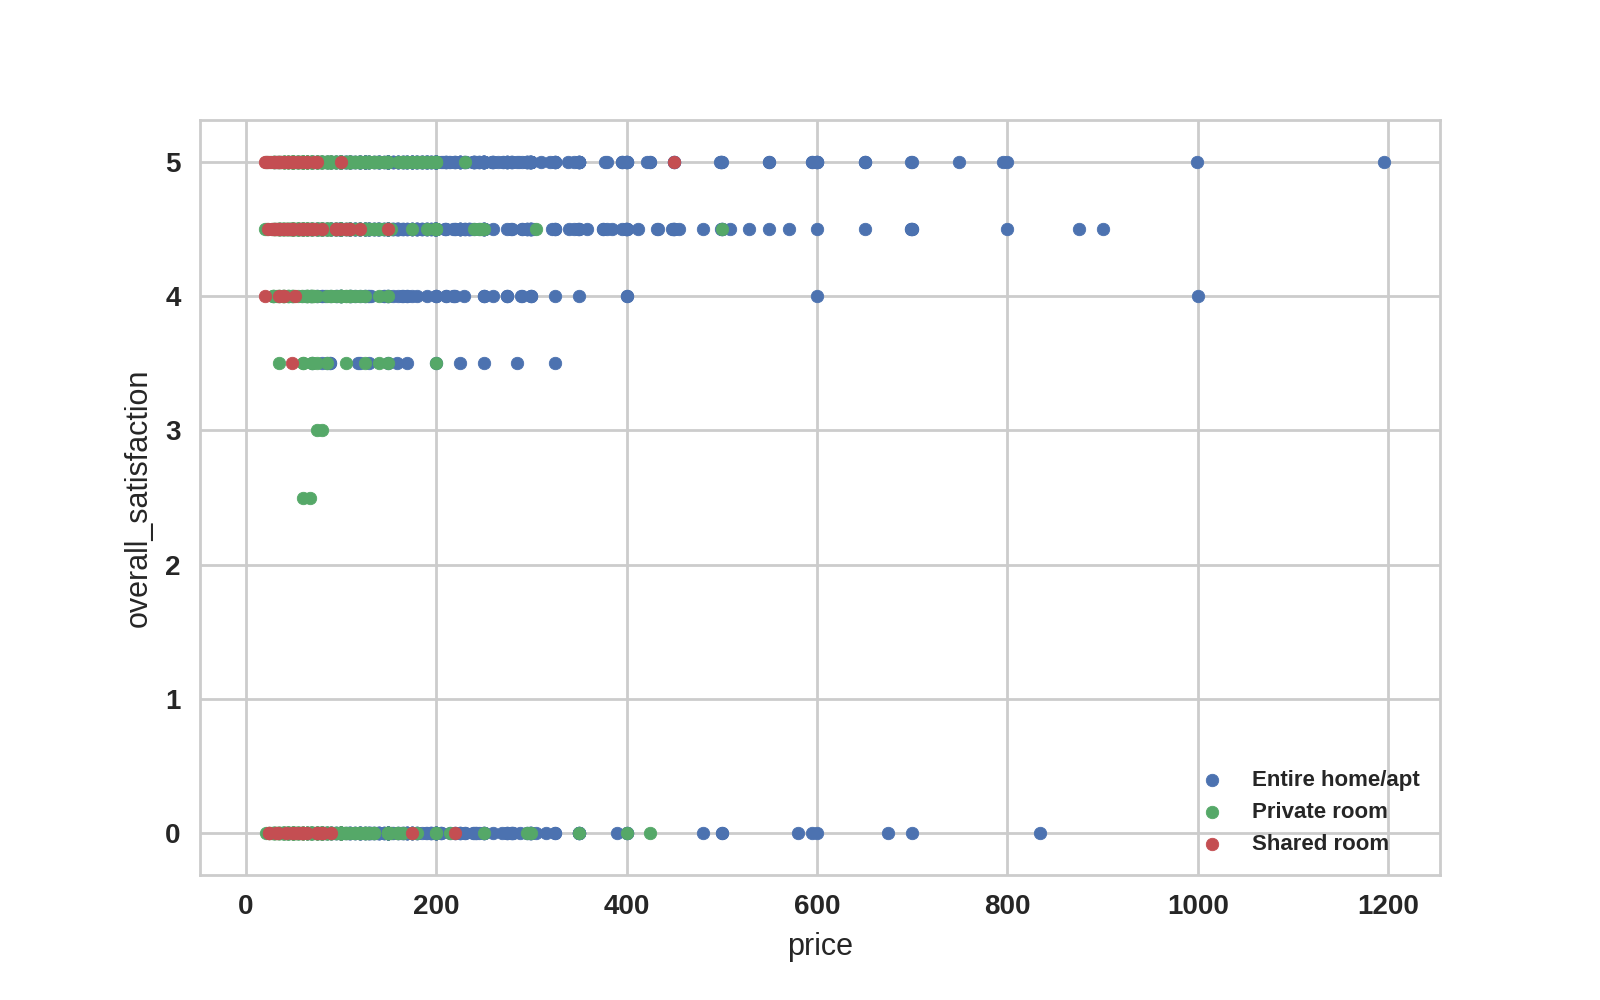
\includegraphics[width = 0.8\textwidth]{images/pair-over-price2.png}
\caption{A 2D-projection on to the satisfiction and price with room type label}
\label{fig:pair-over-price2}
\end{figure}
\begin{figure}[htb]
\centering
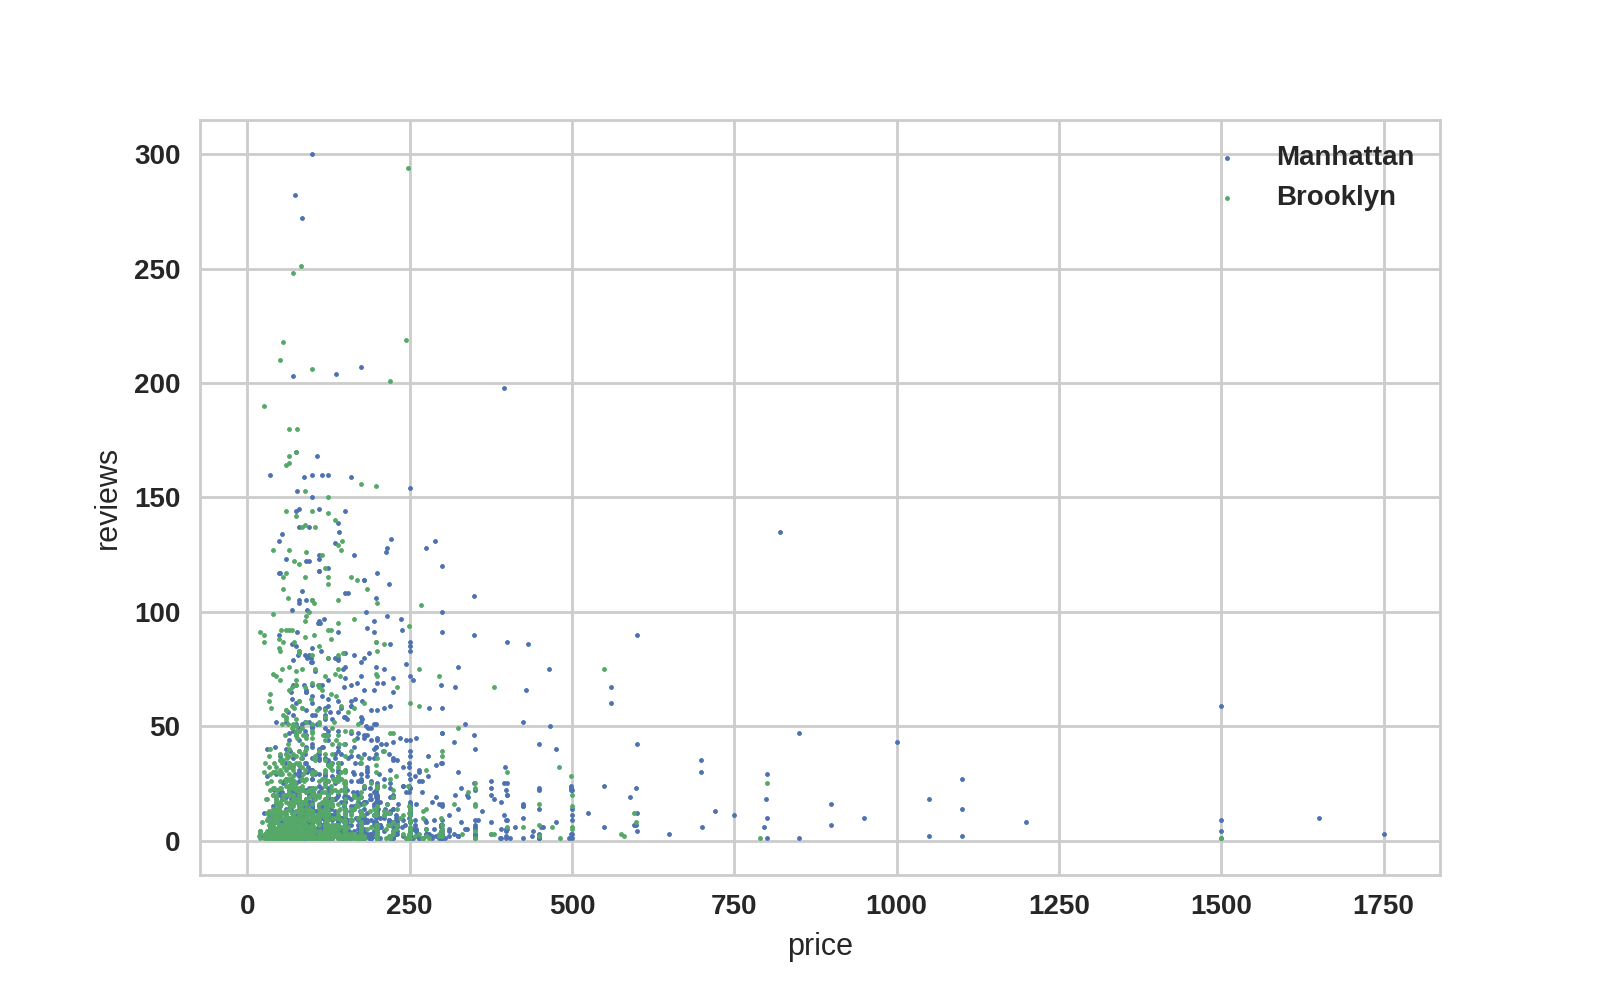
\includegraphics[width = 0.8\textwidth]{images/pair-reviews-price1.png}
\caption{A 2D-projection on to the number of reviews and price with borough label}
\label{fig:pair-reviews-price1}
\end{figure}
\begin{figure}[htb]
\centering
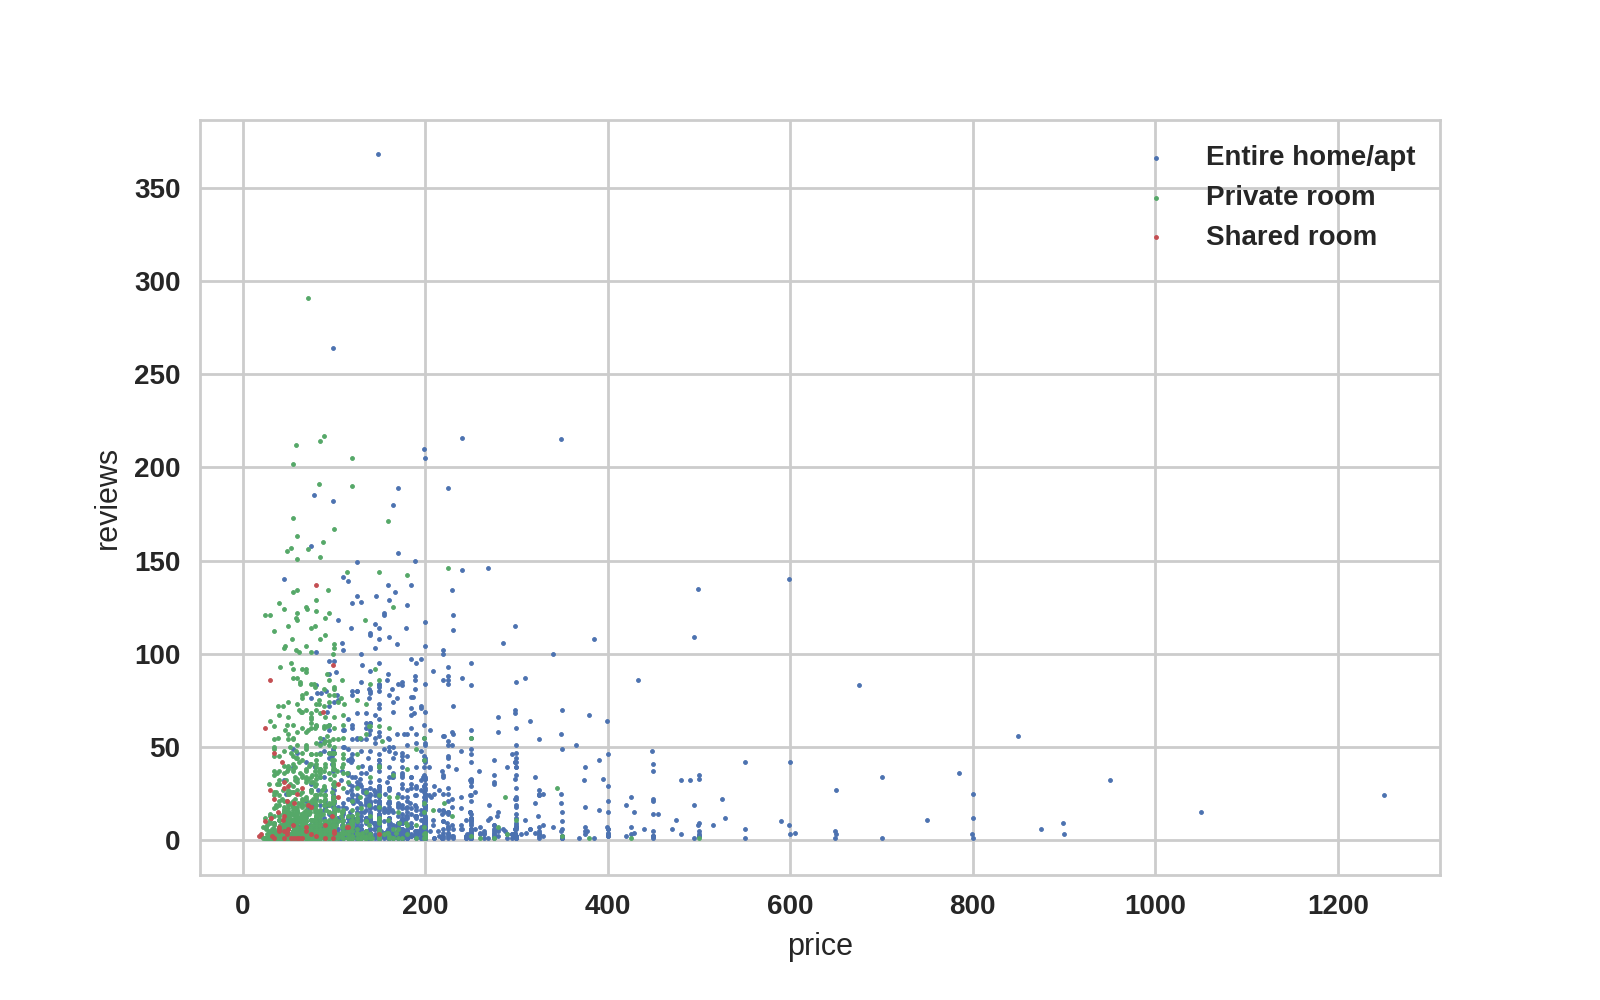
\includegraphics[width = 0.8\textwidth]{images/pair-reviews-price2.png}
\caption{A 2D-projection on to the number of reviews and price with room type label}
\label{fig:pair-reviews-price2}
\end{figure}
%%%%%%%%%%%%%%%%%%%%%%%%%%%%%%%%% figures %%%%%%%%%%%%%%%%%%%%%%%%%%%%%%%%%%%%%%%
\subsection{Principal Component Analysis}
\subsubsection{Prices of the rooms}

It can be noticed from Fig.\ref{fig:eigenvalues1} that the distribution of variance of the principle components is not concentrated to the first serval principal components very well. Thus, if the data is projected on to the first two or three principle components, it can be predicted that the structure of results will not very similar to that of the original data.\par
However, the PCA technique indeed reduce some dimensions, as it can be concluded from the Fig.\ref{fig:eigenvalues1} that the first 15 eigenvectors can preserve the 90\% of the variance of the dataset. 

\begin{figure}[htb]
\centering
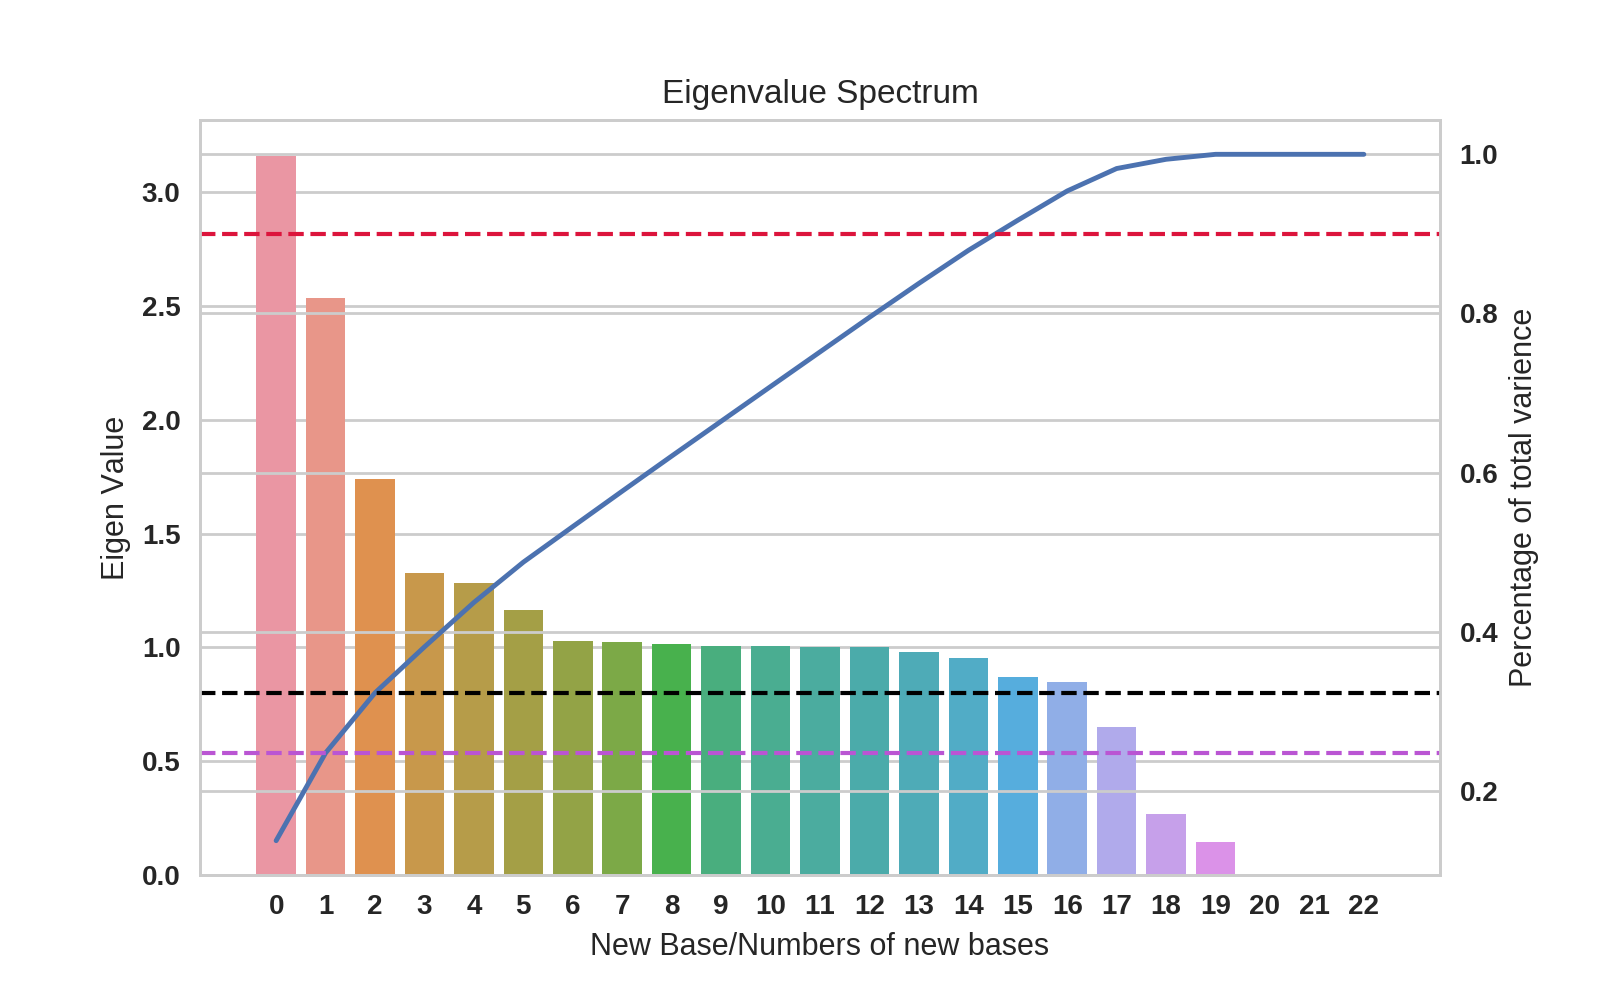
\includegraphics[width = 0.8\textwidth]{images/eigenvalues1.png}
\caption{ A scree plot showing the percentage variance of each principle component, and a running cumulative total}
\label{fig:eigenvalues1}
\end{figure}
\par Figure \ref{fig:pca1-2d} projects the 23 dimensional data onto a sub-space spanned by the first and second eigenvector of the covariance matrix of $X$
\par The more detialed infomation of the first three eigenvectors are shown in the Table \ref{tab:eigenvectors1}.
In the first eigenvector the importance of borough is very important, this is why it can be discovered that in the following PCA projection figues there are 2 similar part of cluster (such as in Fig. \ref{fig:pca1-2d} and \ref{fig:pca1-3d}). Also, the latitude and longtitude are actully related to the borough it located in, thus they increase the distinction or distance in the projection. \par
The price differences are mainly interpreted by the second principal eigenvector. The most siginificant components in the 2nd vector is the room type. Since ``Entire'' type and ``Private'' type are negtive and positive respectively, we can conclude from the PCA projection result that the prices of Entire home/apt rooms are higher much higher than those of Private room. Also, the more accommodates and bedrooms, the higher price the room will have. The importance of accommodate numbers is greater than that of room numbers. And the overall stasifcation does influence a little on the price, which reveal the ``effect of market''.\par
For the 3rd most siginificant eigenVector, the point is that the room with larger value has lower price. So this vector illustrate the property type influence on the price. The price of property type from lower to higher is apartment, house, loft and townhouse.
%%%%%%%%%%%%%%%%%%% PCA1 %%%%%%%%%%%%%%%%%%%%%%
\begin{figure}[htb]
\centering
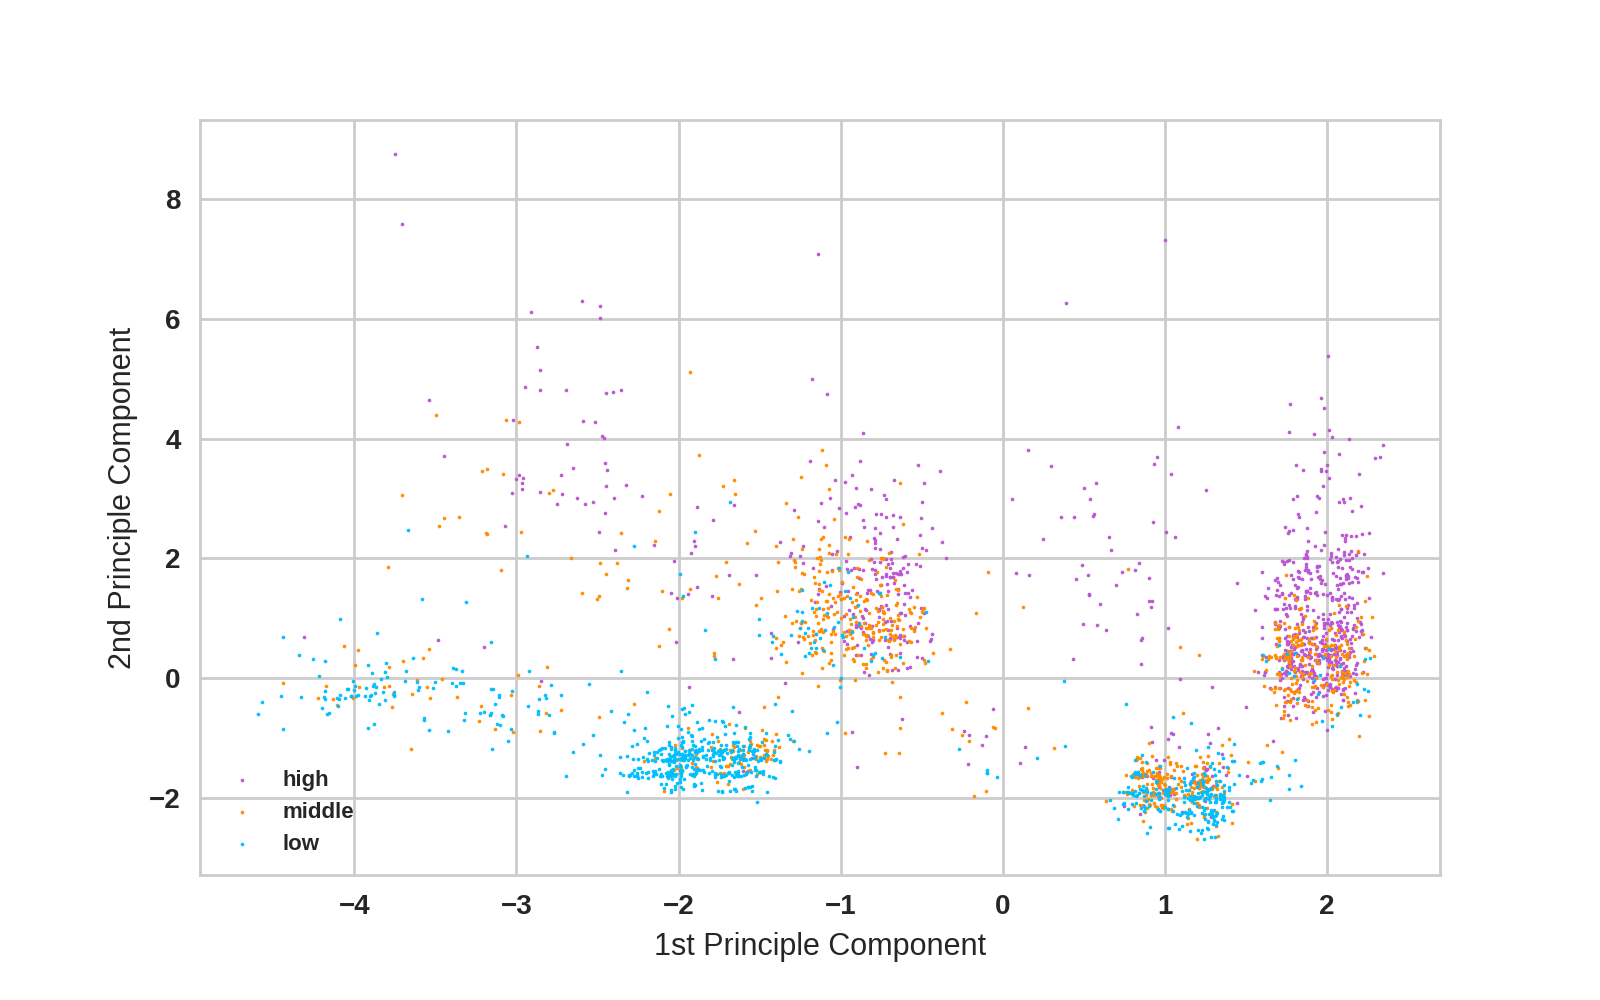
\includegraphics[width = 0.8\textwidth]{images/pca1-2d.png}
\caption{A 2D projection of the PCA results}
\label{fig:pca1-2d}
\end{figure}
\begin{figure}[htb]
\centering
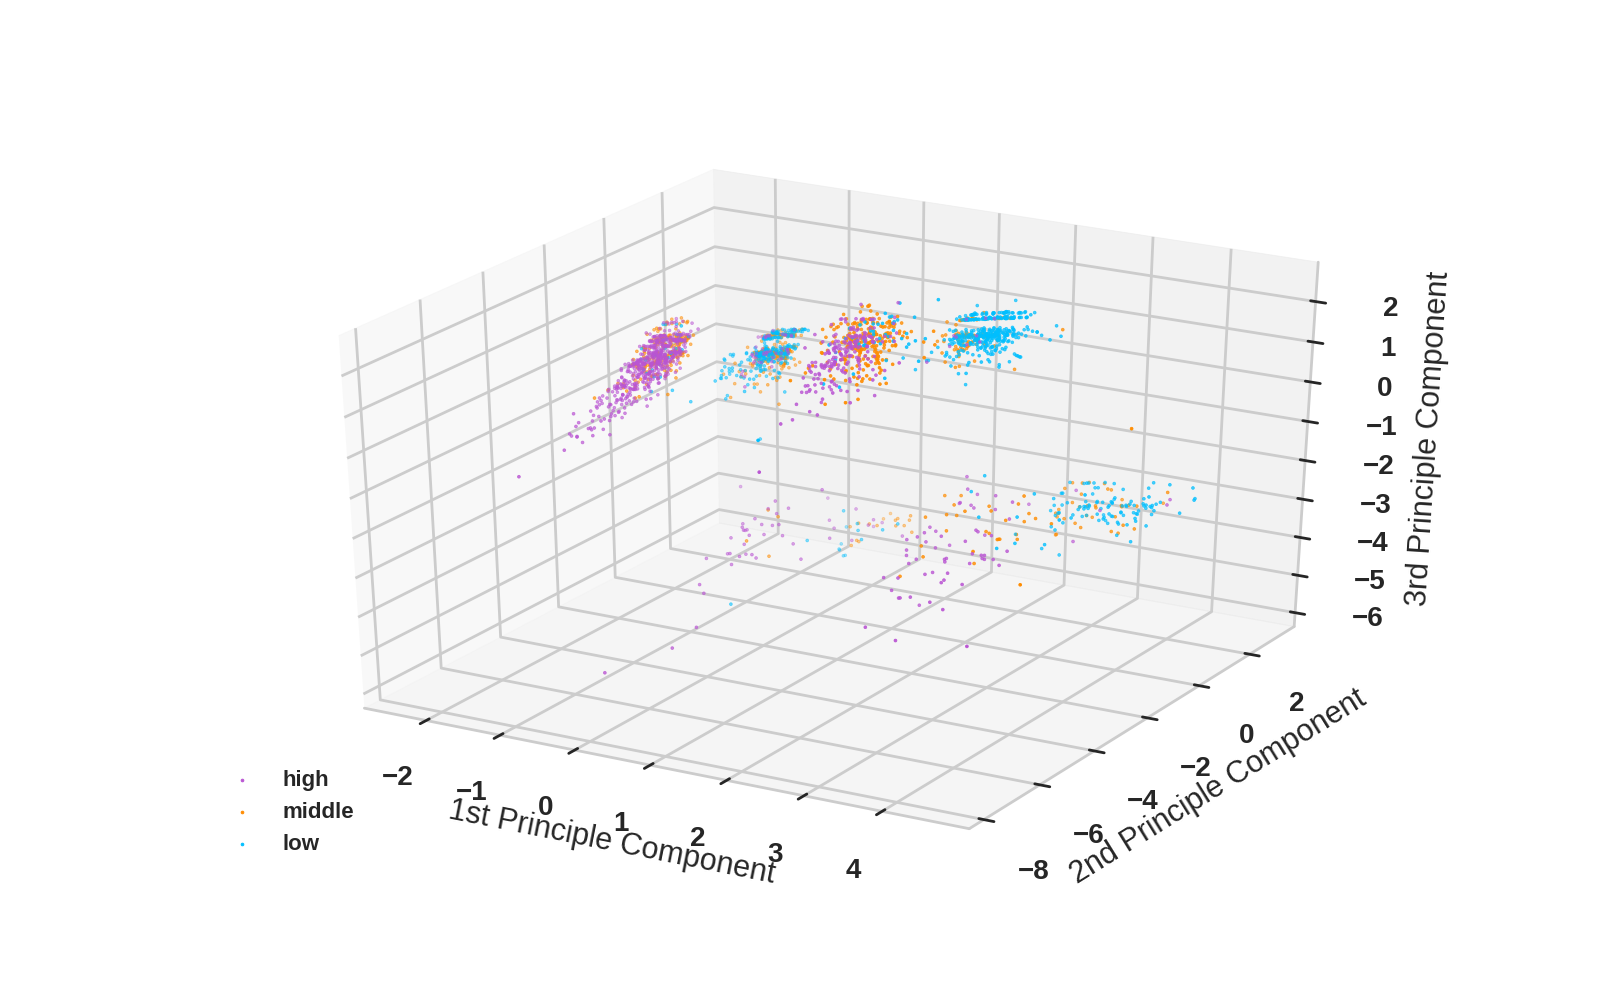
\includegraphics[width = 0.8\textwidth]{images/pca1-3d.png}
\caption{A 3D projection of the PCA results}
\label{fig:pca1-3d}
\end{figure}
% Please add the following required packages to your document preamble:
% \usepackage{booktabs}
\begin{table}[]
\centering
\resizebox{\linewidth}{!}{
\begin{tabular}{@{}crcrcr@{}}
\multicolumn{2}{c}{\begin{tabular}[c]{@{}c@{}}1st Principle Component\\ Eignenvalue 3.15901473\end{tabular}} & \multicolumn{2}{c}{\begin{tabular}[c]{@{}c@{}}2nd Principle Component\\ Eigenvalue 2.53613192\end{tabular}} & \multicolumn{2}{c}{\begin{tabular}[c]{@{}c@{}}3rd Principle Component\\ Eigenvalue 1.73809388\end{tabular}} \\ \midrule
borough\_Manhattan                                           & -0.51484551                                   & room\_type\_Entire home/apt                                  & -0.52678505                                  & property\_type\_Apartment                                    & 0.60738014                                   \\
borough\_Brooklyn                                            & 0.51484551                                    & room\_type\_Private room                                     & 0.51272818                                   & property\_type\_House                                        & -0.36991721                                  \\
latitude                                                     & -0.41706656                                   & accommodates                                                 & -0.50934697                                  & property\_type\_Loft                                         & -0.28433712                                  \\
property\_type\_Apartment                                    & -0.29132238                                   & bedrooms                                                     & -0.34241624                                  & borough\_Manhattan                                           & -0.26485932                                  \\
longitude                                                    & 0.26209607                                    & overall\_satisfaction                                        & -0.14247044                                  & borough\_Brooklyn                                            & 0.26485932                                   \\
property\_type\_House                                        & 0.25374459                                    & latitude                                                     & 0.11644046                                   & latitude                                                     & -0.22556836                                  \\
room\_type\_Private room                                     & 0.15672518                                    & reviews                                                      & -0.0980652                                   & property\_type\_Townhouse                                    & -0.20936499                                  \\
room\_type\_Entire home/ap                                   & -0.15512859                                   & property\_type\_Apartment                                    & 0.09209157                                   & room\_type\_Entirehome/apt                                   & 0.1495919                                    \\
property\_type\_Loft                                         & 0.10969607                                    & longitude                                                    & 0.08412272                                   & property\_type\_Other                                        & -0.14047292                                 
\end{tabular}}
\caption{Details of top three eigenvectors}
\label{tab:eigenvectors1}
\end{table}
%%%%%%%%%%%%%%%%%%% PCA1 %%%%%%%%%%%%%%%%%%%%%%
\subsubsection{Overall satisfaction}
Then the same technique is applied to the infomation without overall satisfection data.
%%%%%%%%%%%%%%%%%%% PCA2 %%%%%%%%%%%%%%%%%%%%%%
\begin{figure}[htb]
\centering
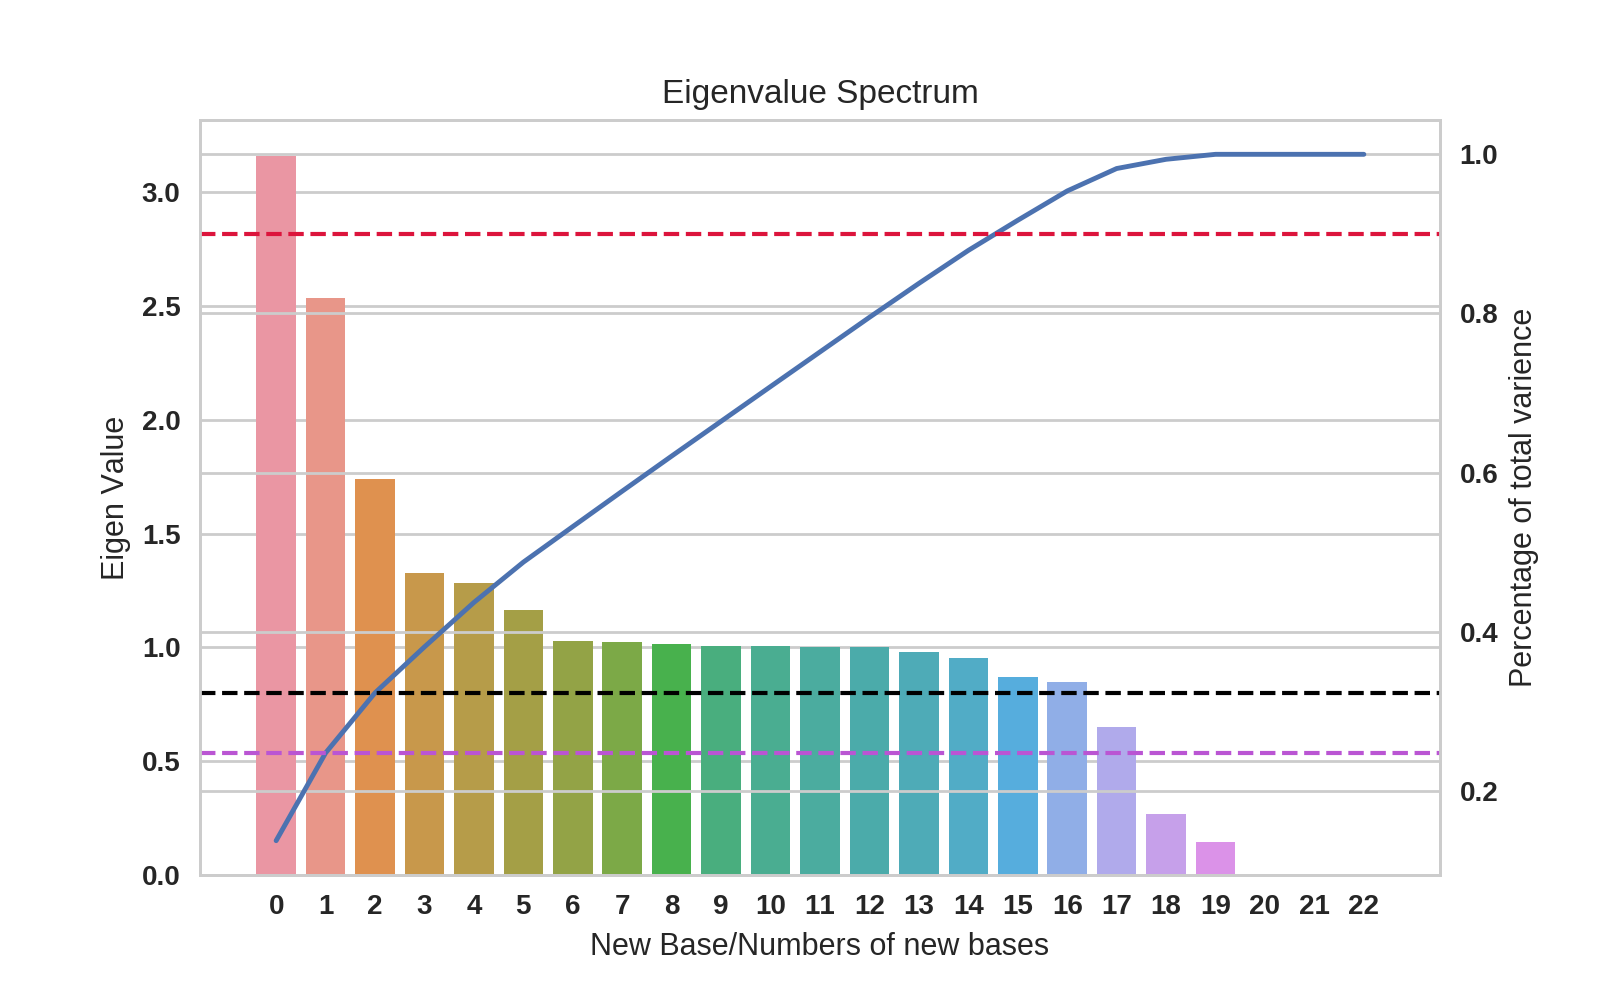
\includegraphics[width = 0.8\textwidth]{images/eigenvalues2.png}
\caption{ A scree plot showing the percentage variance of each principle component, and a running cumulative total}
\label{fig:eigenvalues1}
\end{figure}
\begin{figure}[htb]
\centering
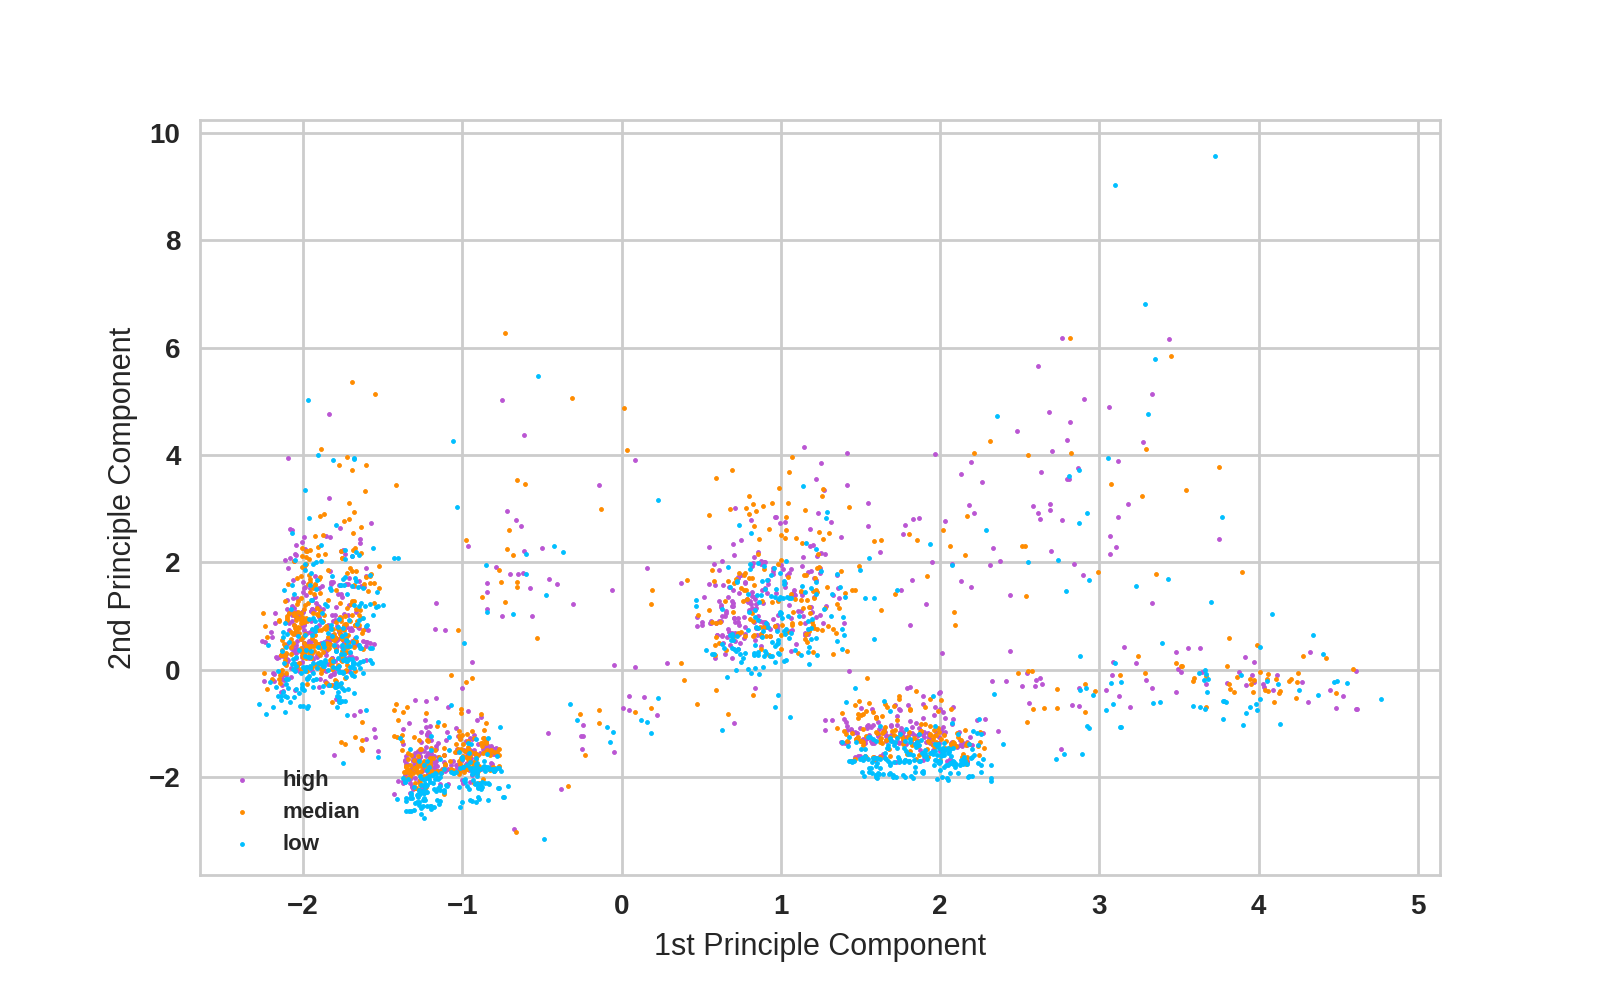
\includegraphics[width = 0.8\textwidth]{images/pca2-2d.png}
\caption{A 2D projection of the PCA results}
\label{fig:pca2-2d}
\end{figure}
\begin{figure}[htb]
\centering
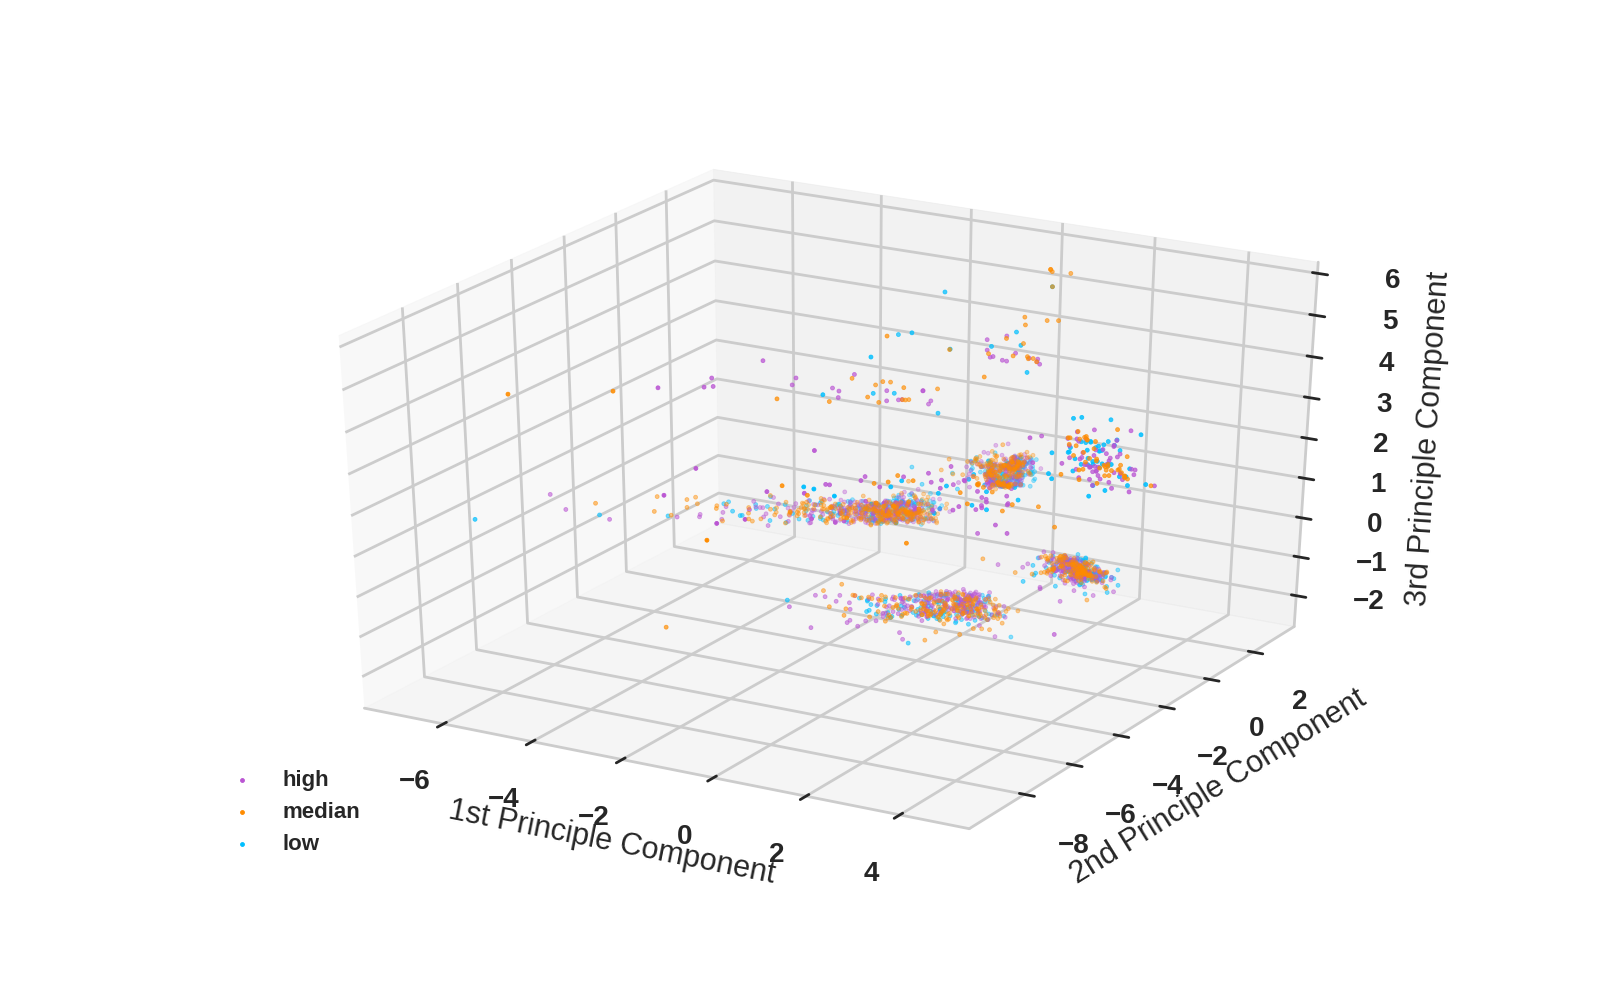
\includegraphics[width = 0.8\textwidth]{images/pca2-3d.png}
\caption{A 3D projection of the PCA results}
\label{fig:pca2-3d}
\end{figure}
%%%%%%%%%%%%%%%%%%% PCA2 %%%%%%%%%%%%%%%%%%%%%%
\subsection{Clustering}

\subsection{Self-orgnization map}


Each cell is the normalised sum of the distances between a neuron and its neighbours.

\subsection{Differences between two boroughs}
\section{Conclusion}

\newpage
\bibliography{biblist}

\end{document}